\subsection{Leapfrog}
    First, we define two function \textit{kick}  and \textit{drift}, which
    we will use to update the velocity and position of the particles, 
    respectively. When updating the position, the periodicity of the system 
    needs to be respected. \\
    \begin{lstlisting}
        void kick(particle * p, int ntot, double dt) {
          for (int i=0; i < ntot; i++){
            for (int k=0; k<3; k++){
              p[i].vel[k] += p[i].acc[k] * dt;
            }
          }
        }
        
        void drift(particle * p, int ntot, double boxsize, double dt) {
          for (int i=0; i < ntot; i++){
            for (int k=0; k<3; k++){
              p[i].pos[k] += p[i].vel[k] * dt;
        
              while (p[i].pos[k] >= boxsize){
                p[i].pos[k] -= boxsize;
              }
              while (p[i].pos[k] < 0){
                p[i].pos[k] += boxsize;
              }
            }
          }
        }
        }\end{lstlisting}

\newpage
\subsection{Potential and kinetic energies}
    \begin{equation}
        T=\frac{1}{k_B}\langle E_\textnormal{kin}\rangle \qquad
        \Rightarrow T'=\langle E_\textnormal{kin}'\rangle
    \end{equation}
    The energies can be calulated using the following \textit{C} code: \\
    \begin{lstlisting}
        void calc_energies(particle *p, int ntot, double *ekin, double *epot) {
          double sum_pot = 0, sum_kin = 0;
        
          for (int i = 0; i < ntot; i++) {
            sum_pot += p[i].pot;
            for(int k = 0; k < 3; k++) {
              sum_kin += p[i].vel[k] * p[i].vel[k];
            }
          }
        
          *ekin = 0.5 * sum_kin / ntot;
          *epot = 0.5 * sum_pot / ntot;
        }\end{lstlisting}
    This leads to the following plot:
    \begin{figure}[h!]
        \centering
        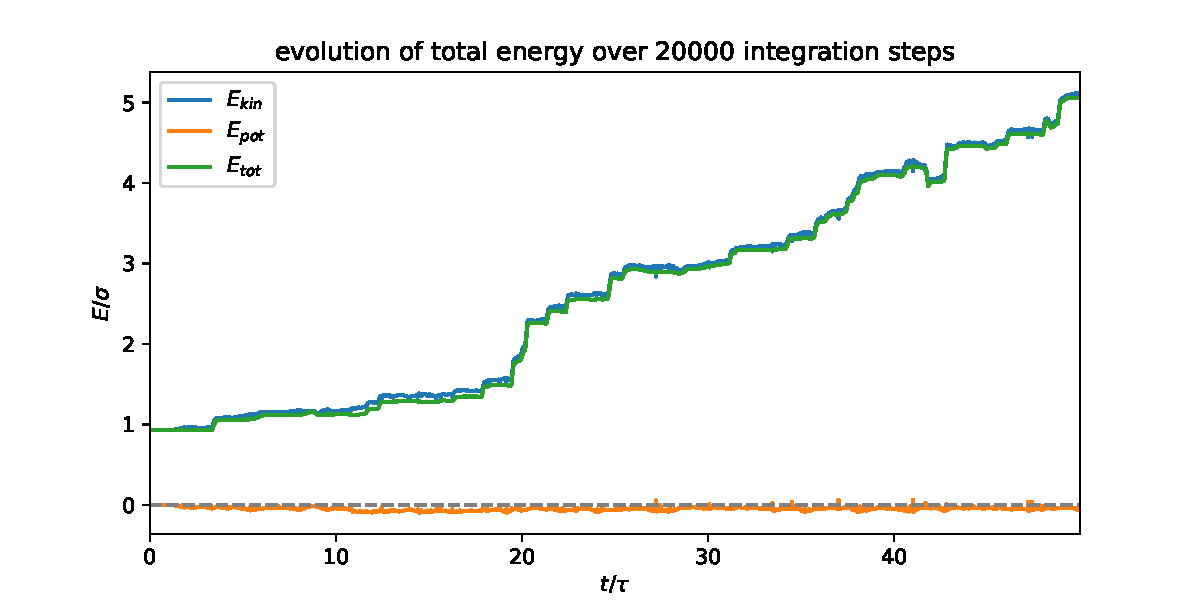
\includegraphics[width=\textwidth]{../figures/energy.pdf}
    \end{figure} \ \\ 
    The potential energy stays relatively constant with only small fluctuations,
    but there is a positive trend in the kinetic (and thus total) energy.
    In between those jumps, the energy stays relatively constant though.
    The jumps might be related to events where two particles occupy 
    positions which are very close to each other.
    We tested this by adjusting the code such that interactions
    between very close particles are ignored.
    Setting a minimum distance $d_{min}=0.1$ leads to smaller jumps than with 
    $d_{min}=0.01$, which again are smaller than without setting $d_{min}$ at 
    all (i.e. taking all interactions into account). This suggests that the 
    jumps might indeed have something to do with these close-encounter 
    events.
    % \begin{figure}[h!]
    %     \centering
    %     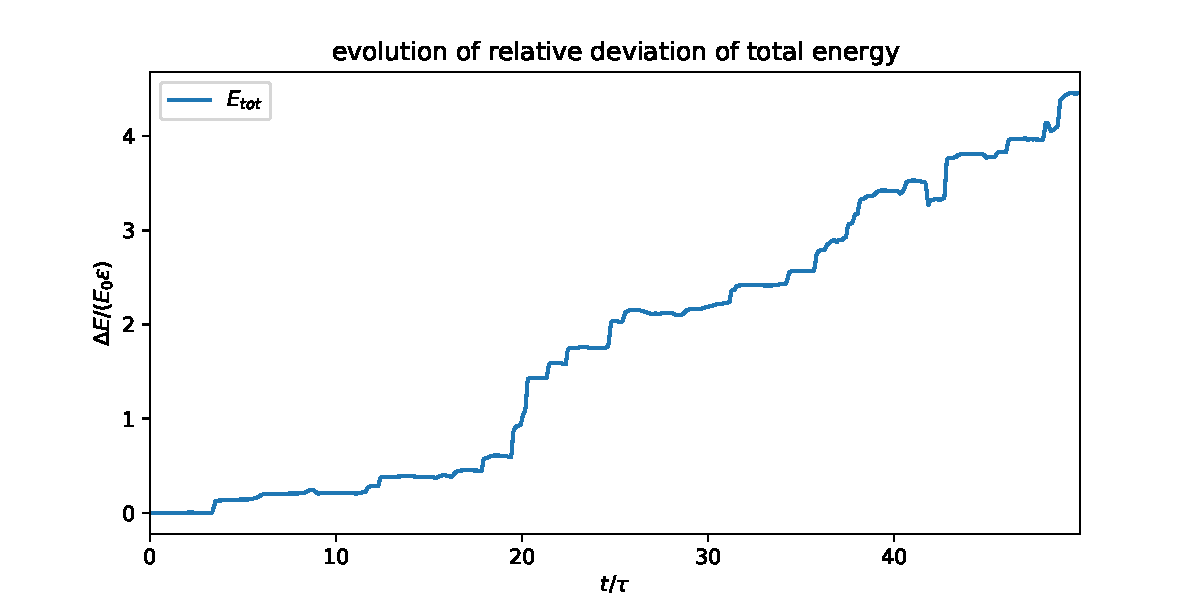
\includegraphics[width=\textwidth]{../figures/relative_energy.pdf}
    % \end{figure} \ \\ 
    % \begin{figure}[h!]
    %     \centering
    %     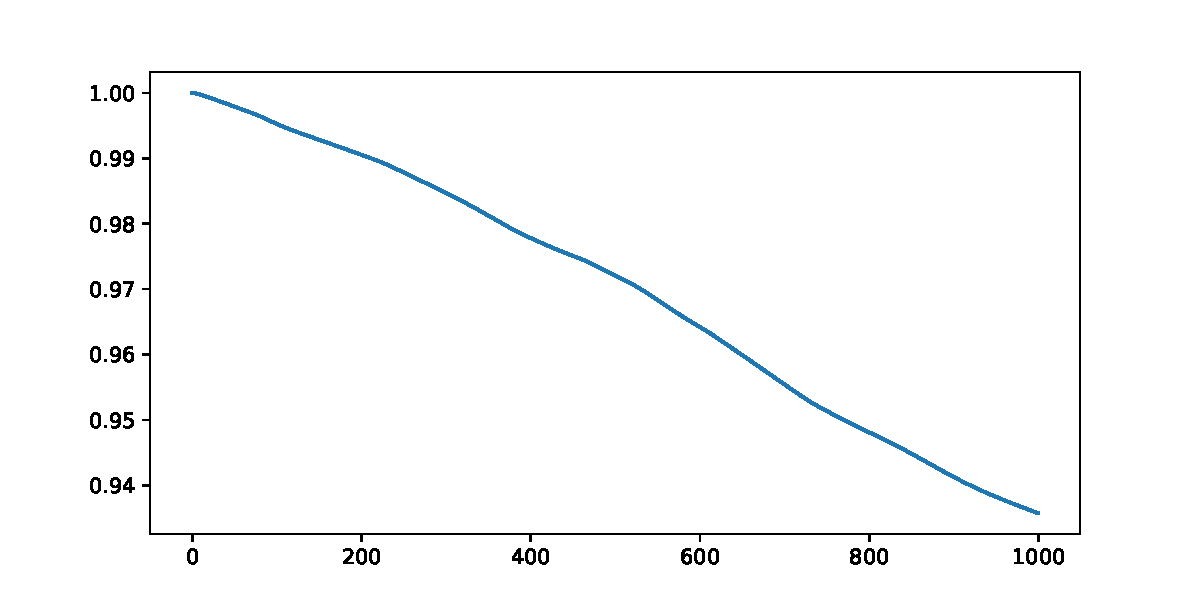
\includegraphics[width=\textwidth]{energy_AC.pdf}
    % \end{figure} \ \\ 

\subsection{20000 time steps}
    For some reason, the computation time increases very fast with rising 
    number of integration steps. For 2000 steps, it takes about 2 seconds,
    for 5000 steps, it takes about 10 seconds, but for 20000 steps we've 
    left the simulation running for over an hour and it still was not finished.
    Thus, we unfortunately could not work on the remaining exercises.

